\documentclass{article}

% Packages
%\usepackage[utf8]{inputenc} % Required for German umlauts
\usepackage{amsmath, bm}
% SVG
\usepackage{svg}
% Bib
\usepackage[backend=biber]{biblatex}
\addbibresource{bib/bibliography.bib}
% Geometry
\usepackage{geometry}
\geometry{
  paper=a4paper, % Change to letterpaper for US letter
  inner=2.5cm, % Inner margin
  outer=3.8cm, % Outer margin
  bindingoffset=.5cm, % Binding offset
  top=1.5cm, % Top margin
  bottom=1.5cm, % Bottom margin
}
\usepackage[onehalfspacing]{setspace}
\usepackage{parskip}
%
\usepackage{enumitem} % description alignment

%
% Tikz Setup
%
\usepackage{tikz}
\usetikzlibrary{tikzmark}
%\newcommand{\tikzmark}[2]{
%    \tikz[overlay,remember picture,baseline]
%    \node[anchor=base] (#1) {$#2$};
%}
\usetikzlibrary{positioning}
%
% Font
%
\usepackage{fontspec}
\setmainfont{Palatino Linotype}
%
% Custom commands
%
%
% Definition of custom commands
%
\usepackage{xparse}

%%
%% Define commands for formatting C3srMatrix data members correctly
%%
\NewDocumentCommand{\DataMember}{ m o }
  {
  \ifmmode
     \text{#1}\IfNoValueF{#2}{[#2]}
   \else
     #1\IfNoValueF{#2}{[#2]}
   \fi
  }

\NewDocumentCommand{\V}{o}
  {\DataMember{V}[#1]}
\NewDocumentCommand{\VS}{o}
  {\DataMember{VS}[#1]}
\NewDocumentCommand{\J}{o}
  {\DataMember{J}[#1]}
\NewDocumentCommand{\JS}{o}
  {\DataMember{JS}[#1]}
\NewDocumentCommand{\JP}{o}
  {\DataMember{JP}[#1]}
\NewDocumentCommand{\RS}{o}
  {\DataMember{RS}[#1]}
\NewDocumentCommand{\RP}{o}
  {\DataMember{RP}[#1]}
\NewDocumentCommand{\CI}{o}
  {\DataMember{CI}[#1]}


%%%%%%%
%%%%%%% Begin of document
%%%%%%%

\author{Stanislaw Hüll}
\title{Student Research Project}
\date{2018-11-11}
\begin{document}

\maketitle

\section{Introduction}

  \subsection{Compressed Sparse Row Matrix Storage Format}

    The compressed sparse row (CSR) format is a widely used storage format for sparse matrices. Unlike other popular sparse matrix storage formats such as the diagonal storage format (DIA) the CSR format is not tailored to any special type of matrix but is a general purpose storage format which makes no assumptions about the matrix's shape or its distribution of non-zeros. The CSR format can be considered an improvement to the naive coordinate format (COO) in that each non-zero's row index is no longer explicitly stored \cite{Bell2011}.

    The CSR format consists of three dense arrays. The values array (V) stores the numerical value for each non-zero entry in the matrix while the associated column index is stored in the column-index array (CI). A third array, the row-pointer array (RP), encodes the beginning of each row's section within the values and column-index arrays, i.e. it stores the offset of each row's first non-zero element into the two arrays. By convention the row-pointer array usually also contains an additional element denoting the total number of non-zero elements in the matrix. An example for the CSR format is given in Figure \ref{fig:csr_example}.

    \begin{figure}[ht]
      \centering
      \begin{minipage}{0.4\textwidth}
        \centering
        $$
        \begin{pmatrix}
          \color{red}{\bm{3}} &                     0 &  \color{red}{\bm{4}} &                    0 \\
                            0 & \color{green}{\bm{1}} &                    0 &                    0 \\
                            0 &                     0 & \color{blue}{\bm{7}} & \color{blue}{\bm{8}} \\
        \end{pmatrix}
        $$
      \end{minipage}
      \begin{minipage}{0.4\textwidth}
        \centering
        $$
        \begin{matrix}
          \text{Values}  & : & \color{red}{3} &   \color{red}{4} & \color{green}{1} & \color{blue}{7} & \color{blue}{8} \\
          \text{Column-Indices} & : & \color{red}{0} &   \color{red}{2} & \color{green}{1} & \color{blue}{2} & \color{blue}{3} \\
          \text{Row-Pointers} & : & \color{red}{0} & \color{green}{2} &  \color{blue}{3} &               5 &                 \\
        \end{matrix}
        $$
      \end{minipage}
      \caption{\textbf{Exemplary matrix with corresponding CSR representation.} The array elements are color-coded in red for the first row, green for the second row and blue for the third row.}
      \label{fig:csr_example}
    \end{figure}

    Thus, as previously mentioned, the CSR format optimizes the storage requirements of general sparse matrices with respect to the naive coordinate format (COO) shrinking the size of the third array from one entry per non-zero element to a single entry per row irrespective of the row's number of non-zeros. Furthermore, the existing literature, in part, utilizes a different nomenclature referring to the arrays as A (values array), JA (column-index array) and IA (row-pointer array), respectively \cite{sparskit}.

    The CSR format's salient feature is the contiguousness of the rows' non-zero elements' values and column indices making it particularly well suited for matrix-vector-multiplication utilizing a conventional row-by-column computation scheme due to ideal data locality. Aside of this characteristic storing the non-zero elements row-by-row as opposed to column-by-column is, to a certain degree, arbitrary and thus exist numerical libraries and toolkits such as the Eigen C++ library \cite{eigen:website} or the Harwell-Boeing sparse matrix collection \cite{harwell-boeing} which utilize the CSR format's conjugate, the compressed sparse column format (CSC), as their default means of storing sparse matrices.

    The CSR format serves as a starting point for the C3SR sparse matrix storage format for structured grid matrices which is the focal point of this work.

  \subsection{Structured Grid Matrices}

    Structured grid computations are ubiquitously used for physical simulations in scientific fields such as, for example, computational fluid dynamics, electrodynamics and astrophysics. Generally, a system of partial differential equations is solved by discretization and linearization of the problem which involves generating a grid corresponding to the physical domain in question. A structured grid refers to a mesh whose nodes are logically rectangular, i.e. they are uniquely identified by a tuple of coordinates and v.v., such as $(i, j, k)$ for three dimensions (Figure \ref{fig:structured_grid_example}).

    \begin{figure}[ht]
        \centering
        \vspace{0.5cm}
        \begin{minipage}{0.4\textwidth}
          \centering
          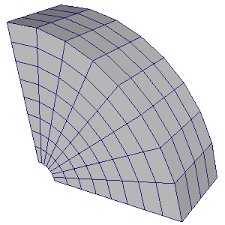
\includegraphics[width=0.9\textwidth]{fig/structured_grid_example.png} % second figure itself
          \caption{\textbf{Curvi-linear grid over a physically complex domain.} The grid nodes are logically rectangular despite the non-rectangular physical domain and thus comprise a structured grid. Source: \cite{daad:website}}
          \label{fig:structured_grid_example}
        \end{minipage}\hfill
        \begin{minipage}{0.5\textwidth}
          \centering
          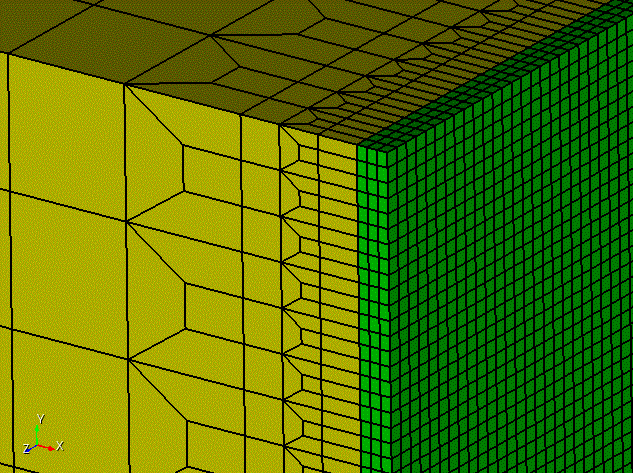
\includegraphics[width=0.9\textwidth]{fig/refined_structured_grid.png} % second figure itself
          \caption{\textbf{Heterogeneous mesh with structured regions.} Outer side (green) and interior volume are fully structured and are connected via an unstructured mesh region. Given proper indexing of grid nodes the resulting sparse matrix will exhibit regularity in the sections pertaining to the structured mesh region. Source: \cite{cubit-mesh-refinement:website}}
          \label{fig:refined_structured_grid}
        \end{minipage}
    \end{figure}

    In contrast to unstructured grids the regularity inherent to structured grids allows for very efficient numerical treatment, such that even in cases where sufficiently complex geometries prohibit the decomposition of the target domain into a single overarching structured grid the domain is often tesselated into an unstructured configuration, with the tiles being filled by independent structured grids \cite{Badcock2000}(Figure \ref{fig:refined_structured_grid}).

    \begin{figure}
        \centering
        \begin{minipage}{0.45\textwidth}
          \centering
          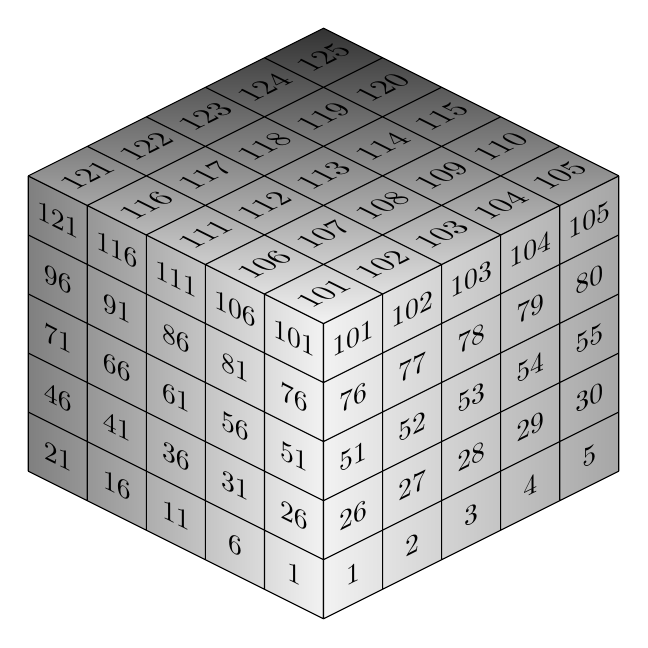
\begin{tikzpicture}[scale=0.75]%[every node/.style={minimum size=1cm},on grid]
\newcommand*{\height}{5}
\newcommand*{\width}{5}
\begin{scope}[every node/.append style={yslant=-0.5},yslant=-0.5]
  \shade[right color=gray!10, left color=black!50] (0,0) rectangle +(\width,\height);

  \foreach \x in {1,...,\width}
    \foreach \y in {1,...,\height}
    {
        \node at (-0.5 + \x, -0.5 + \y) {\pgfmathtruncatemacro\result{21-5*(\x-1)+25*(\y-1)}$\result$};
    }
  \draw (0,0) grid (\height,\width);
\end{scope}
\begin{scope}[every node/.append style={yslant=0.5},yslant=0.5]
  \shade[right color=gray!70,left color=gray!10] (\width,-\height) rectangle +(\height,\width);
    \foreach \x in {1,...,\width}
    \foreach \y in {1,...,\height}
    {
        \node at (\width - 0.5 + \x, -\height + -0.5 + \y) {\pgfmathtruncatemacro\result{1 + 1*(\x-1)+25*(\y-1)}$\result$};
    }

  \draw (\width,-\height) grid (2*\width,0);
\end{scope}
\begin{scope}[every node/.append style={
    yslant=0.5,xslant=-1},yslant=0.5,xslant=-1
  ]
  \shade[bottom color=gray!10, top color=black!80] (2*\width,\height) rectangle +(-\width,-\height);

    \foreach \x in {1,...,\width}
    \foreach \y in {1,...,\height}
    {
        \node at (\width - 0.5 + \x, -0.5 + \y) {\pgfmathtruncatemacro\result{101 + 1*(\x-1)+5*(\y-1)}$\result$};
    }

  \draw (\width,0) grid (2*\width,\height);
\end{scope}
\end{tikzpicture}

        \end{minipage}\hfill
        \begin{minipage}{0.45\textwidth}
            \centering
            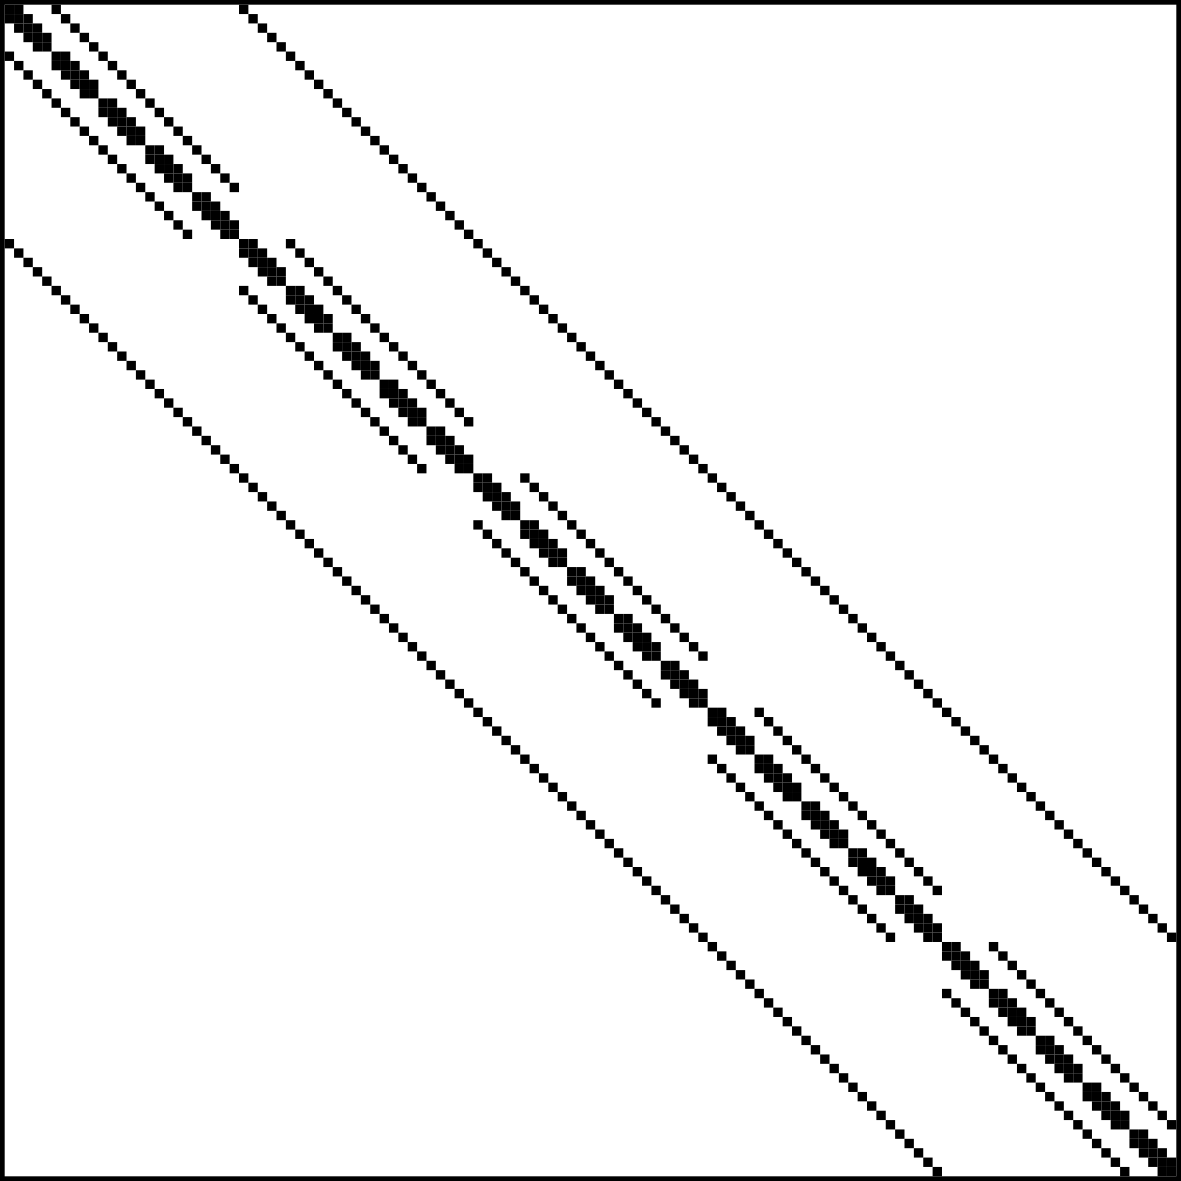
\includegraphics[width=0.9\textwidth]{fig/laplacian_example.png} % second figure itself
        \end{minipage}
        \caption{\textbf{Structured grid and corresponding sparse adjacency matrix for a simple Laplacian} $\nabla^2 u(\vec{r}) = 0$. The Laplace-operator is approximated by the conventional 3-axial symmetric discretization scheme, equivalent to a symmetric 7-point stencil operation.}
        \label{fig:laplacian_example}
    \end{figure}

    The solution procedure yields a sparse linear system whose solution is approximated by iterative methods involving repeated sparse matrix-vector-multiplications $Ax = b$ where the matrix $A$ encodes the adjacency structure of the grid. For a structured grid the resulting matrix's distribution of non-zeros has a very distinct pattern. Generally speaking, such matrices consist of multiple diagonals of non-zero values at fixed intervals while all other elements are zero. The diagonals are almost fully dense with exceptions arising at positions corresponding to nodes at the grid's boundaries, where the regular adjacency pattern of the grid is disturbed by missing nodes. A grid and its corresponding sparse matrix's structure are depicted in Figure \ref{fig:laplacian_example} for a simple Laplacian problem.

    The matrix's non-zero values depend on the underlying physical problem's parameters, the type of PDE and the differential operators' discretization schemes. In general, the non-zeros' numeric values are independent from their location within the matrix but there exist classes of problems where the equivalence of the structure of a set of matrix rows also implies that those rows' non-zeros share the same numeric values. Furthermore, solving problems on higher-dimensional entities such as vectors or matrices yields structured grid matrices whose 'elements' are themselves square matrices \cite{Godwin2013}.

    The sparse matrices relevant to this work areany sparse matrices which contain one or more sets of rows whose non-zero's column indices are identical save for a fixed offset. Structured grid matrices arising from the procedure mentioned above have one such set to which the overwhelming majority of rows belong corresponding to all inner grid nodes (such as in the example in Figure \ref{fig:laplacian_example}). However, all of the ideas presented hereinafter may be applied to any sparse matrix whose structure exhibits any degree of repetiveness.

\section{Threefold Compressed Sparse Row Sparse Matrix Storage Format (C3SR)}

  Evidently, representing a structured grid matrix using the regular CSR format is highly suboptimal, as it has no means of capturing the apparent repetetiveness of the structure. While at first glance the diagonal format might seem an appealing choice for the types of matrices introduced in the previous section, real-life problems produce matrices which are possibly only locally structured, i.e. they contain multiple fully structured sections corresponding to the multiple structured grid regions of the overall heterogeneous domain (Figure \ref{fig:refined_structured_grid}), which need not be aligned in a way to produce a diagonal structure at all. For such matrices the diagonal storage format is highly suboptimal \cite{Bell2011}. Thus a more flexible approach is taken adapting the CSR format to suit the characteristics of structured grid matrices.

  This section introduces the data layout and the matrix-vector multiplication scheme of the threefold compressed sparse row matrix storage format (C3SR). Its aim is to optimize arithmetic performance of matrix-vector multiplications involving structured grid matrices by improving data locality through a structurally-aware space-saving storage scheme and by implementing an efficient arithmetic scheme capable of profiting from modern computer architectures' hardware assets.

  \subsection{Data layout and storage scheme}

    It is cruicial to observe that, in the most general case, the index patterns' regularity is not shared by the non-zero elements' numerical values. While two or more rows may share the same pattern their corresponding values need not be similar to each other at all. To prevent that a lack of common regularity impedes optimizing the storage requirements of one or the other it is hence necessary to decouple the representation of a row's non-zeros column index positions from the representation of their numerical values. The C3SR format accounts for this circumstance and maintains separate data structures for the non-zeros' column indices and their values.

    Based on the observation that structured grid matrices contain many rows whose non-zeros are located at the same positions except for a possible offset the C3SR format decomposes the column-index positions into the column index of the row's first non-zero element, referred to as the row's peg hereinafter, and the relative column indices of all of the row's non-zeros with respect to the first non-zero's column index, i.e. the relative offsets with respect to the peg index. The latter column index offsets relative to the peg index shall be called the row's column index pattern, or simply the row's pattern. Naturally, only unique patterns are stored, drastically shrinking the storage requirements of such matrices whose majority of rows exhibit the same pattern.

    Thus, in order to represent the column indices of a matrix row's non-zeros the C3SR format utilizes three arrays:

    \begin{description}[align = left, labelwidth = 4cm]
      \item [JP - \emph{Peg column index}] \hfill \\
        Column index of each row's first non-zero. One element per row in matrix.
      \item [J - \emph{Column index patterns}] \hfill \\
        Column index position offsets of the rows' non-zeros relative to peg column index for each row. Only unique patterns are stored.
      \item [JS - \emph{Pattern index pointer}] \hfill \\
        Index pointer to each row's first element within \J. One element per row in matrix.
    \end{description}

    An example matrix and its corresponding structural information are given in Figure \ref{fig:c3sr_example_structure}.

    \begin{figure}[ht]
      \centering
      \begin{minipage}{0.4\textwidth}
        \centering
        $$
        \begin{pmatrix}
          0 & \bullet & 0 & \bullet & \bullet & 0 \\
          0 & \bullet & 0 & 0 & \bullet & 0 \\
          0 & 0 & \bullet & 0 & \bullet & \bullet \\
        \end{pmatrix}
        $$
      \end{minipage}
      \begin{minipage}{0.4\textwidth}
        \centering
        $$
        \begin{matrix}
          \JP & : & 1 & 0 & 2 &   &   \\
           \J & : & 0 & 2 & 3 & 0 & 3 \\
          \JS & : & 0 & 3 & 0 &   &   \\
        \end{matrix}
        $$
      \end{minipage}
      \caption{\textbf{Matrix with corresponding C3SR representation (structural information only).} The non-zeros are denoted as black dots. The $0^{\text{th}}$ and $2^{\text{th}}$ row exhibit the same column index pattern $\big(0,2,3\big)$ at different peg index positions of $1$ and $2$, respectively, thus the $0^{\text{th}}$ and the $2^{\text{th}}$ element of \JS point \J[0], which is the first element of this unique pattern. The $1^{\text{th}}$ row has a unique pattern which is stored after the previous pattern within \J at offset $3$ which \JS[1] accordingly points.}
      \label{fig:c3sr_example_structure}
    \end{figure}

    The matrix's non-zeros' numerical values are represented using two dense arrays \V, which contains the values and \VS, the index-pointer into \V which relates to \V in the same way \JS relates to \J. If multiple rows exhibit the same pattern and their values match at the same time the values are stored only once within \V which allows for efficient matrix-vector multiplication schemes shown below.

    \begin{description}[align = left, labelwidth = 4cm]
      \item [\V - \emph{Values}] \hfill \\
        Non-zeros' numerical values. Duplicates across rows with same pattern are stored only once.
      \item [\VS - \emph{Values Index Pointer}] \hfill \\
        Index pointer to each row's first element within \V. One element per row in matrix.
    \end{description}

    A sixth and final array \RS stores the number of non-zeros in each row of the matrix. This information is required as the index-pointer arrays \JS and \VS point a row's first element within \J and \V but may not contain the information about how long the segment pertaining to the row within those arrays is.

    \begin{description}[align = left, labelwidth = 4cm]
      \item [\RS - \emph{Row Size}] \hfill \\
        Number of non-zeros for each row. One element per row in matrix.
    \end{description}

    Another exemplary matrix and its full C3SR format representation are given in Figure \ref{fig:c3sr_example_full}.

    \begin{figure}[ht]
      \centering
      \begin{minipage}{0.4\textwidth}
        \centering
        $$
        \begin{pmatrix}
          1 & 2 & 0 & 3 & 0 & 0 \\
          0 & 1 & 2 & 0 & 3 & 0 \\
          0 & 0 & 4 & 5 & 0 & 0 \\
          0 & 0 & 6 & 7 & 0 & 0 \\
        \end{pmatrix}
        $$
      \end{minipage}
      \begin{minipage}{0.4\textwidth}
        \centering
        $$
        \begin{matrix}
          \JP & : & 0 & 1 & 2 & 2 &   &   &   \\
           \J & : & 0 & 1 & 3 & 0 & 1 &   &   \\
          \JS & : & 0 & 0 & 3 & 3 &   &   &   \\
           \V & : & 1 & 2 & 3 & 4 & 5 & 6 & 7 \\
          \VS & : & 0 & 0 & 3 & 5 &   &   &   \\
         \RS & : & 3 & 3 & 2 & 2 &   &   &   \\
        \end{matrix}
        $$
      \end{minipage}
      \caption{\textbf{Matrix with corresponding full C3SR representation.} The $0^{\text{th}}$ and $2^{\text{th}}$ rows exhibit the same pattern and the same values, thus the values are stored only once. The last two rows also share a common pattern with different values.}
      \label{fig:c3sr_example_full}
    \end{figure}

    /TODO? Nomenclature section after abstract?
    /TODO: 3fold -compression erklären :p

  \subsection{Matrix-Vector Multiplication Schemes} \label{subsec:matrix-vector-multiplication-schemes}

    // TODO: Intro text

    \subsubsection{Basic CSR-like Multiplication Scheme} \label{subsubsec:basic-csr-like-multiplication-scheme}

      Algorithmically, the basic row-by-column matrix-vector multiplication scheme of the C3SR format is similar to that of the CSR format (Figure \ref{fig:c3sr_matvecmult_basic}). Differences arise only in the C3SR's additional offset $\JP[k]$ which is applied to each relative column index prior to accessing the argument vector $x$.

      As the C3SR format utilizes additional arrays to store index-pointers the number of memory accesses increases likewise. Assuming a general case of a large sparse matrix devoid of any regularity in its structue whose size exceeds the machine's cache the CSR format's arithmetic performance will be better proportional to the reduction of loads from memory with respect to the C3SR format as this is a memory bound computation involving few trivial arithmetic operations.

      \begin{figure}[ht]
        \centering
        $$
        \begin{matrix}
          \text{CSR}  & : & \sum \limits_{\alpha = 0}^{\RP[k+1] - \RP[k] - 1} & \bigg( & \V[\RP[k] + \alpha]   & \cdot & x\big[\CI[\RP[k] + \alpha]\big] & \bigg)\\
          \vspace{0.3cm} \\
          \text{C3SR} & : & \sum \limits_{\alpha = 0}^{\RS[k] - 1} & \bigg( & \V\big[\VS[k] + \alpha\big] & \cdot & x\bigg[\J\big[\JS[k] + \alpha\big] + \JP[k]\bigg] & \bigg) \\
        \end{matrix}
        $$
        \caption{\textbf{Matrix-vector multiplication schemes of C3SR and CSR format in comparison.} The $k^{\text{th}}$ component of the product $Ax$ is shown. The C3SR format accesses \V and \J from their dedicated index-pointer arrays while the CSR format utilizes one common row-pointer array. Additionally, the C3SR format requires the relative column indices to be offset by the peg column index for each row.}
        \label{fig:c3sr_matvecmult_basic}
      \end{figure}

      On the flipside, structured matrices facilitate very compact storage allowing a small segment of memory, corresponding to possibly only a few cache lines, to contain the matrix's complete structural information and, depending on the underlying physical problem, even the numeric values. This can drastically improve arithmetic performance of the C3SR format despite the more complex memory access scheme, as will be shown in the benchmark section.

    \subsubsection{Vectorized SIMD Multiplication Scheme} \label{subsubsec:vectorized-simd-multiplication-scheme}

      In addition to the performance gain utilizing the basic multiplication scheme due to better data locality the data layout of a structured matrix in C3SR format allows for the matrix-vector multiplication to be implemented utilizing SIMD parallelism. The matrix's data is layed out in memory in such a way that the matrix-vector multiplication may be performed for multiple rows at a time using vectorization. Depending on the composition of the matrix corresponding to the types of problems mentioned in the introduction three different but very similar multiplication schemes can be devised.

      Suppose that a horizontal slice of rows $r, \ldots, r+k$ has diagonal structure with the diagonals starting at indices $s, t, \ldots $, such as is depicted in Figure \ref{fig:simd_scheme_diag}. The matrix-vector multiplication for each of the slice's rows is composed of the same number of summands, one per diagonal. Each of the summands is a product of the diagonal's non-zero entry and the argument's corresponding element, starting out with $a_{r,s} \cdot x_s$ for the first diagonal's initial element and $a_{r,t} \cdot x_t$ for the second diagonal. For each subsequent row the matrix element's indices are incremented aswell as the argument vector's index, commencing with $a_{r+1, s+1} \cdot x_{s+1}$ for the first diagonal's second element and accordingly for each other diagonal.

      As each diagonal's summand accesses the argument vector's elements in consecutive fashion, for example $x_s, x_{s+1}, \ldots, x_{s + k}$ for the first diagonal, the multiplication can be vectorized. The other summand's constituents, the diagonal's elements, are accessed at a fixed offset which is equal to the number of diagonals. This is due to the fact that the matrix slice's non-zero elements are stored row-by-row, where each row has the same number of elements. Thus $a_{r,s}$ is located as many elements before $a_{r+1, r+2}$ within \V as there are diagonals.

      In SIMD terms a stride-gather and a load is required for the diagonal's elements and the argument vector, respectively. The two vector registers are then multiplied and the result is then added onto the next product pertaining to the subsequent diagonal.

      \begin{figure}[ht]
        \centering
        $$
        \begin{pmatrix}
          \\
          \cdots & 0 & a_{r,s} & 0 & \cdots & a_{r,t} & 0 & \cdots & \cdots & \cdots \\
          \cdots & \cdots & 0 & a_{r+1,s+1} & 0 & \cdots & a_{r+1,t+1} & 0 & \cdots & \cdots \\
          \cdots & \cdots & \cdots & 0 & a_{r+2,s+2} & 0 & \cdots & a_{r+2,t+2} & 0 & \cdots \\
          \\
        \end{pmatrix}
        $$
        $$
        \begin{matrix}
          \begin{bmatrix}
            a_{r,s}     \\
            a_{r+1,s+1} \\
               \vdots   \\
            a_{r+k,s+k} \\
          \end{bmatrix} & \cdot & \begin{bmatrix}
                                    x_s      \\
                                    x_{s+1}  \\
                                      \vdots \\
                                    x_{s+k}  \\
                                  \end{bmatrix} & + & \begin{bmatrix}
                                                      a_{r,t}     \\
                                                      a_{r+1,t+1} \\
                                                        \vdots    \\
                                                      a_{r+k,t+k} \\
                                                      \end{bmatrix} & \cdot & \begin{bmatrix}
                                                                                x_t \\
                                                                                x_{t+1} \\
                                                                                \vdots \\
                                                                                x_{t+k}
                                                                              \end{bmatrix} & + & \cdots & = \begin{bmatrix}
                                                                                                                 y_{r} \\
                                                                                                                 y_{r+1} \\
                                                                                                                 \vdots \\
                                                                                                                 y_{r+k}
                                                                                                                \end{bmatrix}\\

        \end{matrix}
        $$
        %$$
        %\V: \begin{pmatrix}
        %  \ldots & a_{r,s} & a_{r,t} & \ldots & a_{r+1,s+1} & a_{r+1,t+1} & \ldots & a_{r+2,s+2} & a_{r+2,t+2} & \ldots \\
        %\end{pmatrix}
        %$$
        \caption{\textbf{Matrix slice with diagonal structure and corresponding vectorized matrix-vector-multiplication scheme.} Each diagonal's elements are located within \V at a fixed stride offset corresponding to the number of diagonals. Depending on the hardware capabilities this may make the gather-load operation more efficient.}
        \label{fig:simd_scheme_diag}
      \end{figure}

      For the case of a matrix slice whose structure is diagonal and whose values within each diagonal are identical, e.g. $a_{r,s} = a_{r+1, s+1} = \ldots$ for the first diagonal etc., the multiplication scheme is simplified in that the argument vector's values contained in the vector register are simply scaled by the diagonal's value instead of being subjected to a vectorized multiplication (Figure \ref{fig:simd_scheme_diag_collated}).

      \begin{figure}[ht]
        \centering
        $$
        \begin{pmatrix}
          \\
          \cdots & 0 & a_{r,s} &  0 & \cdots & a_{r,t} & 0 & \cdots & \cdots & \cdots \\
          \cdots & \cdots & 0 & a_{r+1,s+1} & 0 & \cdots & a_{r+1,t+1} & 0 & \cdots & \cdots \\
          \cdots & \cdots & \cdots & 0 & a_{r+2,s+2} & 0 & \cdots & a_{r+2,t+2} & 0 & \cdots \\
          \\
        \end{pmatrix}
        $$
        %$$
        %\V: \begin{pmatrix}
        %  \ldots & a_{r,s} & a_{r,t} & \ldots & \ldots \\
        %\end{pmatrix}
        %$$
        $$
        \begin{matrix}
          a_{r,s} & \cdot & \begin{bmatrix}
                                    x_s      \\
                                    x_{s+1}  \\
                                      \vdots \\
                                    x_{s+k}  \\
          \end{bmatrix} & + & a_{r,t} & \cdot & \begin{bmatrix}
                                                x_t \\
                                                x_{t+1} \\
                                                \vdots \\
                                                x_{t+k}
                                                                              \end{bmatrix} & + & \cdots & =  \begin{bmatrix}
                                                                                                                 y_{r} \\
                                                                                                                 y_{r+1} \\
                                                                                                                 \vdots \\
                                                                                                                 y_{r+k}
                                                                                                                \end{bmatrix}
        \end{matrix}
        $$
        \caption{\textbf{Matrix slice with diagonal structure and uniform values and corresponding vectorized matrix-vector-multiplication scheme.} In addition to the diagonal structure the matrix row's values are identical simplifying the arithemtic scheme.}
        \label{fig:simd_scheme_diag_collated}
      \end{figure}

      The third practically relevant case are matrix slices whose structure is uniform, i.e. each row's non-zero elements are situated at the same columns. The corresponding vectorized matrix-vector multiplication scheme is again similar to the general case of a diagonal structure. Here the argument vector's elements serve as scaling constants for the vector register containing the matrix's elements, which are again located at fixed stride-offsets within \V. Note that for matrices stemming from structured grid computations the values necessarily differ inbetween rows as the matrix would be singular otherwise.

      \begin{figure}[ht]
        \centering
        $$
        \begin{pmatrix}
          \\
          \cdots & 0 & a_{r,s} &  0 & \cdots & a_{r,t} & 0 & \cdots \\
          \cdots & 0 & a_{r+1,s} & 0 & \cdots & a_{r+1,t} & 0 & \cdots \\
          \cdots & 0 & a_{r+2,s} & 0 & \cdots & a_{r+2,t} & 0 & \cdots \\
          \\
        \end{pmatrix}
        $$
        %$$
        %\V: \begin{pmatrix}
        %  \ldots & a_{r,s} & a_{r,t} & \ldots & a_{r+1,s} & a_{r+1,t} & \ldots & a_{r+2,s} & a_{r+2,t} & \ldots \\
        %\end{pmatrix}
        %$$
        $$
        \begin{matrix}
          \begin{bmatrix}
            a_{r,s}     \\
            a_{r+1,s} \\
               \vdots   \\
            a_{r+k,s} \\
          \end{bmatrix} & \cdot & x_s & + & \begin{bmatrix}
                                              a_{r,t}     \\
                                              a_{r+1,t} \\
                                                \vdots    \\
                                              a_{r+k,t} \\
                                            \end{bmatrix} & \cdot & x_t & + \cdots & = \begin{bmatrix}
                                                                                       y_{r}   \\
                                                                                       y_{r+1} \\
                                                                                       \vdots  \\
                                                                                       y_{r+k} \\
                                                                                     \end{bmatrix}
        \end{matrix}
        $$
        \caption{\textbf{Matrix slice with uniform structure and corresponding vectorized matrix-vector-multiplication scheme.} Each non-zero column's elements are located within \V at a fixed stride offset corresponding to the number of non-zero columns. As in Figure \ref{fig:simd_scheme_diag} this may improve the performance of loading the SIMD register's values from memory.}
        \label{fig:simd_scheme_uniform}
      \end{figure}

      All of the above mentioned arithmetic schemes can be extended to vector registers of arbitrary length and are thus theoretically able to scale with additional hardware cabalities. Of course, in order to utilize the above mentioned computation schemes a preliminary analysis of the matrix's structure has to be performed in order to determine the segments which can facility vectorized arithmetic. Due to the storage scheme of the C3SR format this can be done very cheaply since if a matrix segment has diagonal or uniform structure all of the rows exhibit the same pattern and hence the same values in \JS. For uniformly structured segments all peg indices are identical, while for a diagonally structured segment the peg indices are consecutive integers. Additionally, if the rows' values are identical for the case of a diagonal structure the rows' index-pointers \VS are also identical.

\section{Performance Benchmarks}

  The matrix-vector multiplication performance of the C3SR format is measured in its CSR-like and vectorized implementations (see \ref{subsec:matrix-vector-multiplication-schemes}). Firstly, a baseline performance is established by comparing the matrix-vector multiplication performance of the C3SR format's CSR-like multiplication scheme introduced in \ref{subsubsec:basic-csr-like-multiplication-scheme} against the CSR format's performance on different structured grid matrices and on three different machines. Secondly, the C3SR format's baseline performance is compared against its vectorized counterpart introduced in \ref{subsubsec:vectorized-simd-multiplication-scheme}.

  The following subsection introduce the structured grid matrices used for the performance benchmarks and their method of acquisition. Subsequently, the results of the performance benchmarks are discussed.

  \subsection{Generation of Structured Grid Matrices as Test Matrices}

    For the purpose of gauging the arithmetic performance test matrices are created in CSR format which are then converted to C3SR format. These matrices resemble the structure of the structured grid matrices introduced above and are created by iterating through a 3D grid of fixed integral dimensions X, Y, Z and applying a given stencil operation which encodes the desired adjacency relationship of the grid. Nodes requested by the stencil but missing from the grid, i.e.  nodes on the grid's outer borders are omitted, i.e. their corresponding entries in the adjacency matrix carry a zero which is equivalent to Dirichlet-type boundary conditions.

    The matrix's non-zero entries' numeric values are obtained from evaluating a sinusoidal function at the geometric center point $\vec{r} = (x, y, z)$ inbetween the two nodes in question whereby each Cartesian component $x, y, z$ is scaled by its coordinate's span $X, Y, Z$. An additional offset serves to prevent that entries in the matrix correponding to adjacent nodes according to the stencil incidentally evaluate to 0. The function utilized is $$W(x,y,z; n_x, n_y, n_z) = 2 + \sum \limits_{d \in \{x,y,z\}} \sin{\frac{d}{d_{\text{max}}} \cdot \pi \cdot n_d} $$ where $n_x, n_y, n_z$ are periodicity parameters for each dimensions. The matrix in Figure \ref{fig:laplacian_example} has been created using this method.

    Note that $n_d = 0 \Leftrightarrow \partial_d W(\vec{r}) \equiv 0$, introducing a periodicity in the corresponding dimension $d$. This feature is utilized to control the periodicity in the matrix's values.

    For the purpose of this work two different sets of parameters are utilized generating two different matrices: A smaller matrix generated from a $100 \times 100 \times 100$ grid with the periodicities $n_x = n_y = n_z = 0$ and a second, larger matrix based on the same grid but different periodicities $n_x = 1.1; n_y = 1.2; n_z = 1.3$. Both matrices are generated from a symmetric 7p-stencil operation.

    The first, smaller matrix's values are identical inbetween two rows whose structure is the same, such that \V and \J contain the same number of elements. The second, larger matrix's values are all unique between rows and thus \V contains approximately $7 \cdot 100^3$ elements (Figure \ref{fig:matrix_stats}).

    \begin{figure}[ht]
      \centering
      \begin{tabular}{ l | c c }
          Array & Small Matrix & Large Matrix        \\
        \hline                                       \\
        \V         & $135$          & $6940000$      \\
        \VS        & $1000000$      & $1000000$      \\
        \J         & $135$          & $135$          \\
        \JS        & $1000000$      & $1000000$      \\
        \JP        & $1000000$      & $1000000$      \\
        \RS        & $1000000$      & $1000000$      \\
        Total Size in C3SR format & $\approx 16$MB & $\approx 72$MB \\
        Total Size in CSR Format & $\approx 87$MB & $\approx 87$MB \\
        \hfill
      \end{tabular}
      \caption{\textbf{Matrices in C3SR format used for matrix-vector multiplication benchmarking.} Number of elements is displayed for each array. \V stores double-precision floating-points while all other arrays use 32 bit-wide integers. Additionally, the matrix's size in CSR representation is listed.}
      \label{fig:matrix_stats}
    \end{figure}

    Note that as the two matrices share the same structure and thus their only difference is found in \V and \VS. The small matrix primarily utilizes the second matrix-vector multiplication scheme (Figure \ref{fig:simd_scheme_diag_collated}) while the large matrix mainly relies on the first scheme (Figure \ref{fig:simd_scheme_diag}). The matrices are generated using the asc::matrixgen C++ library\footnote{https://mp-force.ziti.uni-heidelberg.de/asc/AscMatrixGen}.

  \subsection{Performance of CSR-like Matrix-Vector Multiplication}

    The C3SR format's CSR-like matrix-vector multiplication scheme (referred to as \emph{baseline implementation} hereinafter; see \ref{subsubsec:basic-csr-like-multiplication-scheme}) is compared against its CSR format's pendant using the Eigen C++ library \cite{eigen:website} on three different machines using the structured grid matrices introduced in the previous section. The results are displayed in Figure \ref{fig:baseline_arithmetic_performance}.

    \begin{figure}[!ht]
      \centering
      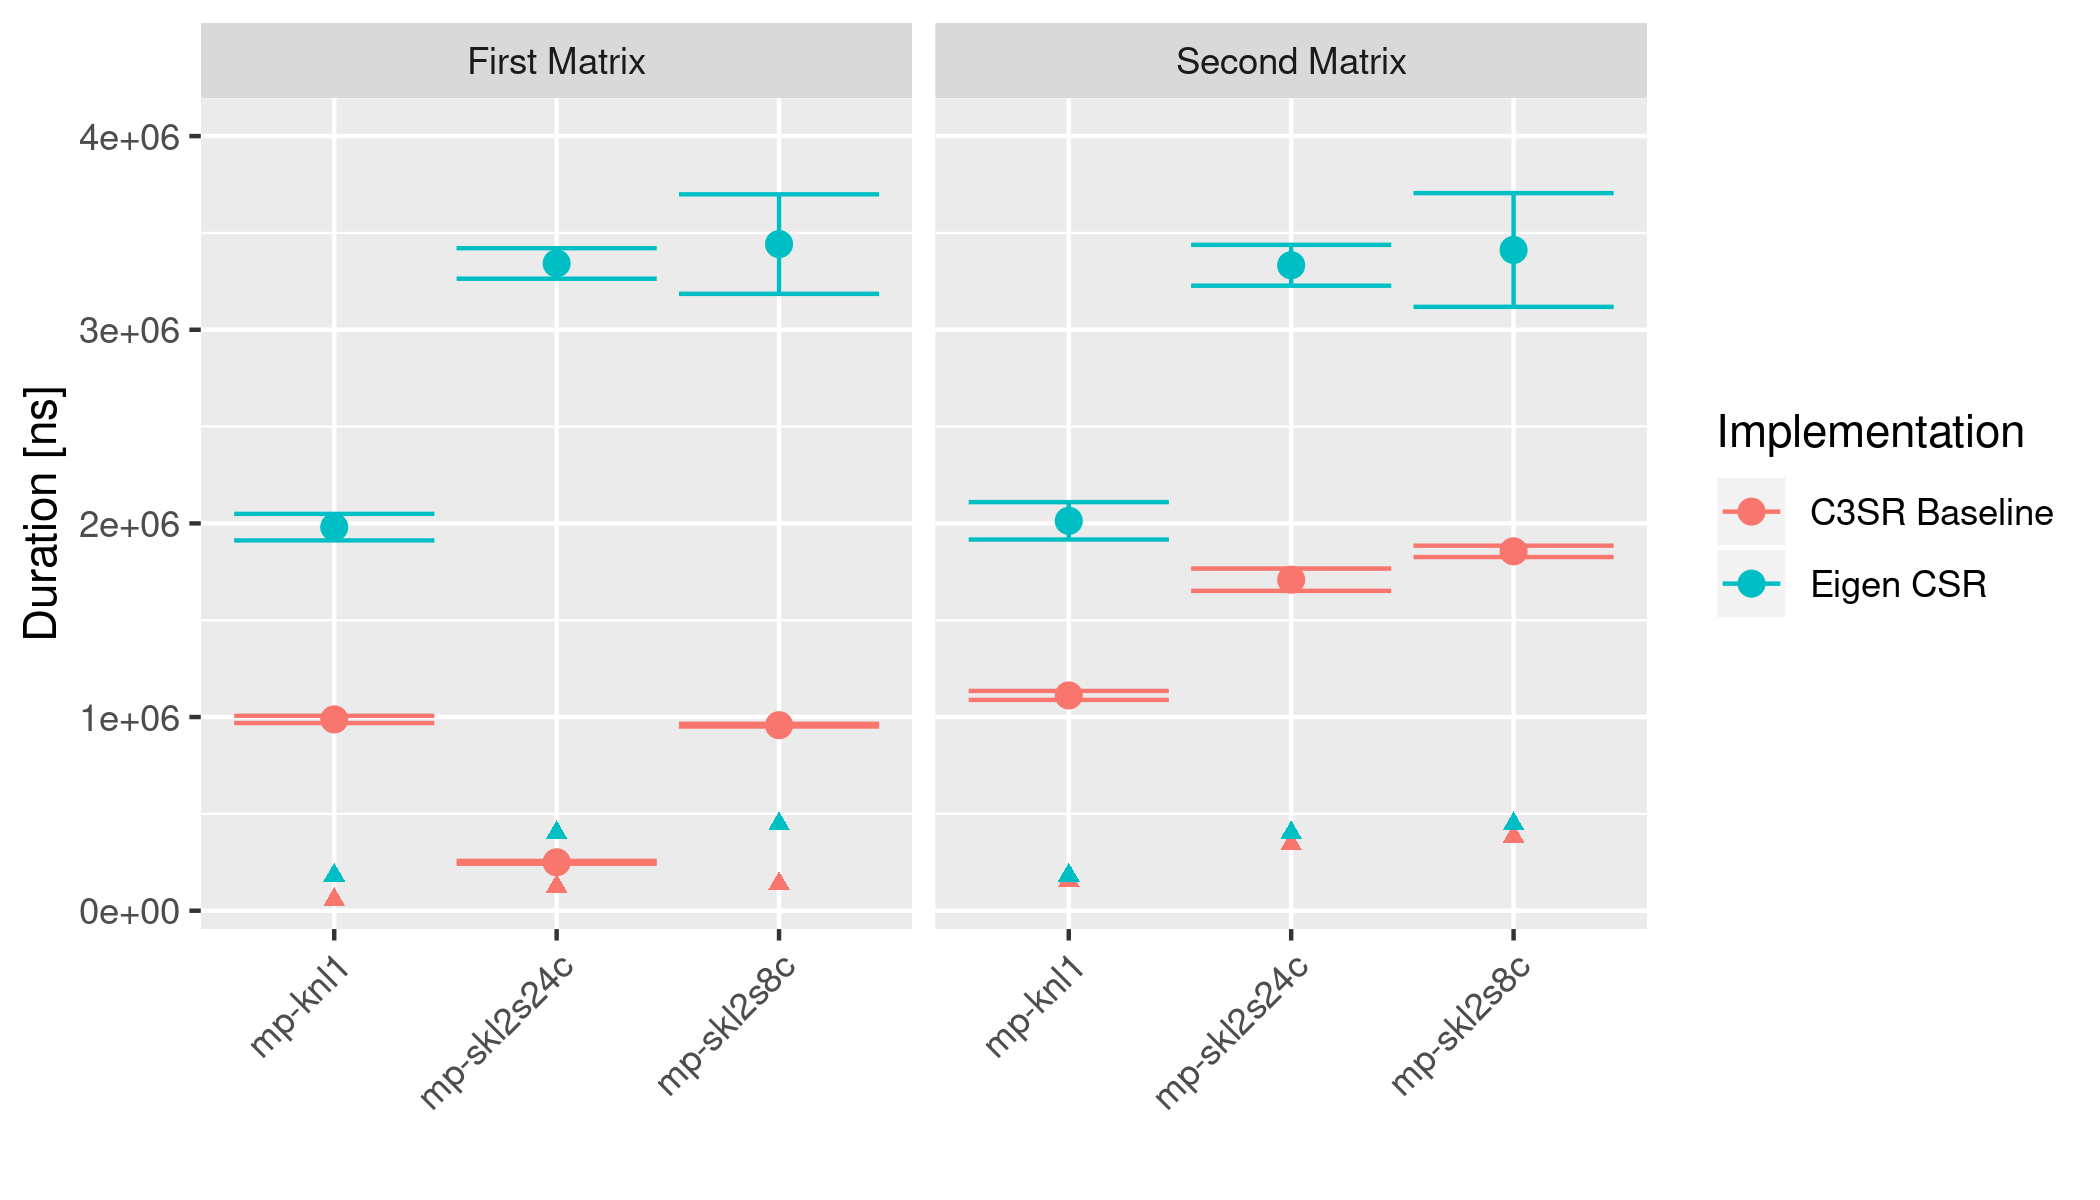
\includegraphics[width=0.9\textwidth]{assets/eigen_vs_c3sr_baseline}
      \caption{\textbf{Performance comparison of the CSR format against the C3SR format on structured grid matrices.} The means and sample standard deviations of $10$ samples à $10000$ consecutive matrix-vector multiplications are shown. As the CSR format's representation of the different matrices is identical except for different numeric values the arithmetic performance is the same save for some minor statistical variance.}
      \label{fig:baseline_arithmetic_performance}
    \end{figure}

    By design of the C3SR format it outperforms the CSR format in the order of magnitude of around $50\%$ irrespective of the machine. This is due to the reduction in size of the representation of the matrices and the consequent improvement in data locality as the C3SR format's arithmetic is slightly more complex as discussed in \ref{subsubsec:basic-csr-like-multiplication-scheme}. Accordingly, the performance improvement is more pronounced for the smaller matrix entailing speed-up factors of roughly 2, 13, and 3.

    + NUMA-aware memory allocation vs CSR uses open-MP (no NUMA) + dynamic overhead.

  \subsection{Performance of SIMD Matrix-Vector Multiplication}

    The C3SR format's matrix-vector multiplication performance is measured using two different implementations: the CSR-like multiplication scheme (\ref{subsubsec:basic-csr-like-multiplication-scheme}, referred to as the 'baseline implementation' hereinafter) is compared against the SIMD multiplication scheme (\ref{subsubsec:vectorized-simd-multiplication-scheme}) on the two different structured grid matrices introduces in the previous section. The implementation of the SIMD multiplication scheme utilizes the explicit SIMD vectorization library UME::SIMD \cite{umesimd2017}. The results are displayed in Figure \ref{fig:arithmetic-performance}.

    \begin{figure}[!ht]
      \centering
      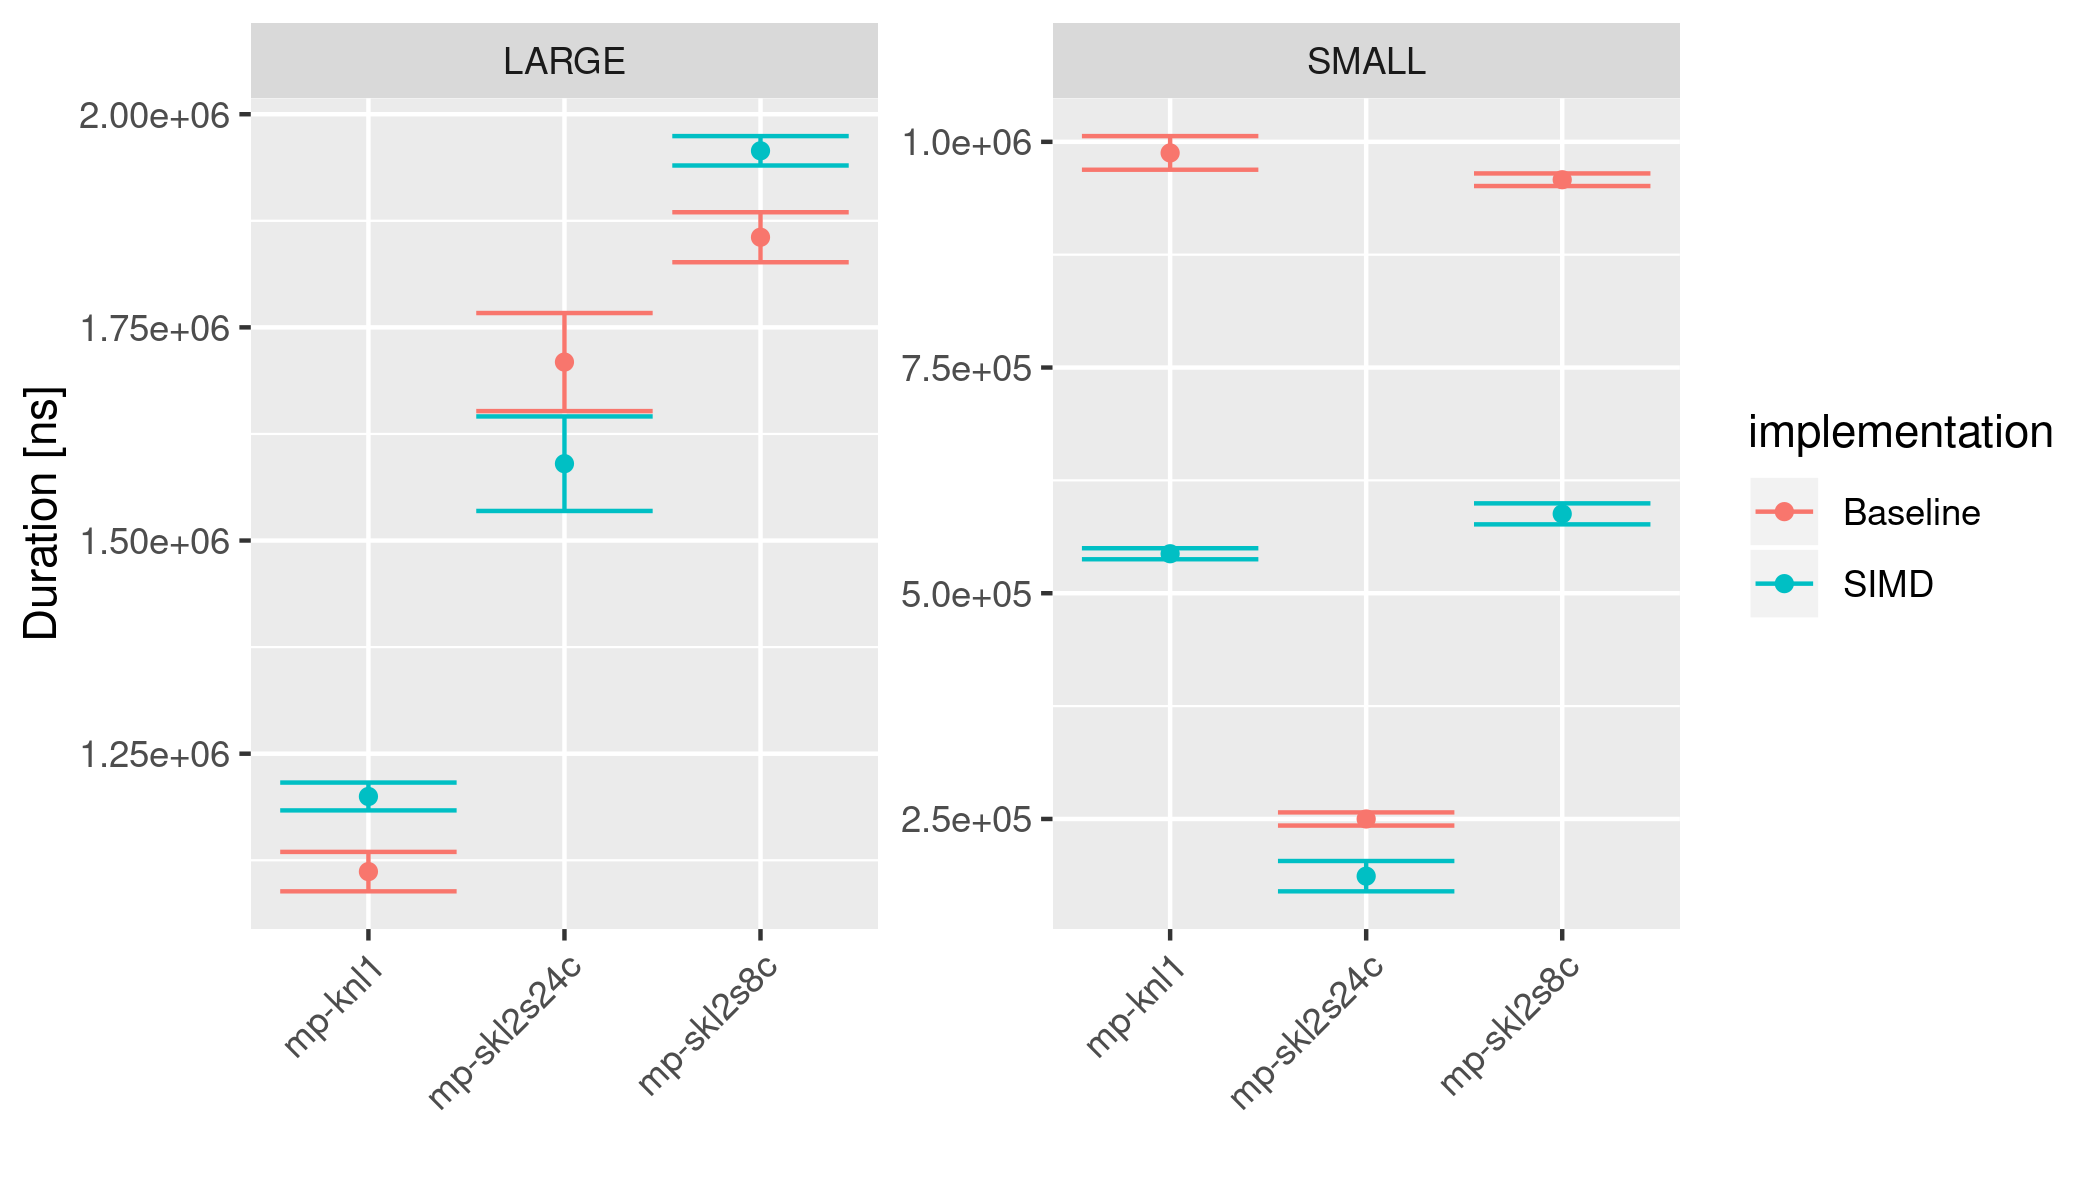
\includegraphics[width=0.9\textwidth]{assets/arithmetic_performance}
      \caption{\textbf{Performance of matrix-vector multiplication.}}
      \label{fig:arithmetic-performance}
    \end{figure}

    Sparse matrix-vector multiplication is a memory-bound computation so that the efficacy of a vectorized arithmetic implementation depends very strongly on the amount of data that is required to be read from memory and whether the dynamic overhead involved in determining the applicable SIMD scheme is compensated by a speed-up in arithmetic. This fact is reflected in the measurements as for the large matrix the SIMD implementation is generally slower than the baseline implementation. Only for the small matrix a significant speed-up can be observed on every machine. However, this might be partly due to the fact that the large matrix's SIMD multiplication scheme is less performant as it involves strided loads from memory which might equate to regular gather operations on the hardware used for this benchmark (see \ref{subsubsec:vectorized-simd-multiplication-scheme}).

  \subsection{Data compression}

  --> As previous section show: Speedup mainly due to reduction in total object size. But reduction costs time --> Diminishing returns;

    This plot compares the number of array elements required in the C3SR format to store a fully structured matrix's column index information (green curve) against the baseline size of the equivalent CSR format matrix's column index array (red curve) depending on the partition size utilized for the structural compression. The C3SR format's recorded number of elements comprises the sum of the sizes of the J, JP and JS arrays, respectively. The RS array and the CSR format's row-pointer array are left out of the consideration as they are identical in size. The underlying $50 \times 50 \times 50$ grid contains $125000$ nodes to which the symmetric 7-pt stencil is applied. The numerical values of the matrix are of no concern for its structure.

    The C3SR format's diminishing storage requirements are caused solely by J (blue curve) as JS and JP are constant in size, each containing $125000$ elements, one per matrix row. The size of J exhibits an inverse linear relationship to the partition size, as can be inferred from the straight line's gradient in the double logarithmic plot. This is due to the fact that large grids mainly consist of inner nodes whose corresponding rows in the matrix all share the same pattern. Hence the overwhelming majority of partitions' column index information will condense to 7 elements within J (and one element per row for JS and JP) irrespective of the partition size with exceptions arising only around the few border nodes and their corresponding rows.

    The minimum size of J is determined by the matrix's unique patterns which correspond to 8 corner nodes a 4 adjacent nodes, 12 edge nodes a 5 adjacency nodes, 6 face nodes a 6 adjaceny nodes and the inner nodes with the full 7 adjacency nodes totalling $135$ entries. (TODO: Tikz 3d-draw representative of all nodes creating unique patterns).

    TODO: Ausreißer erklären.
    \begin{figure}[ht]
      \centering
      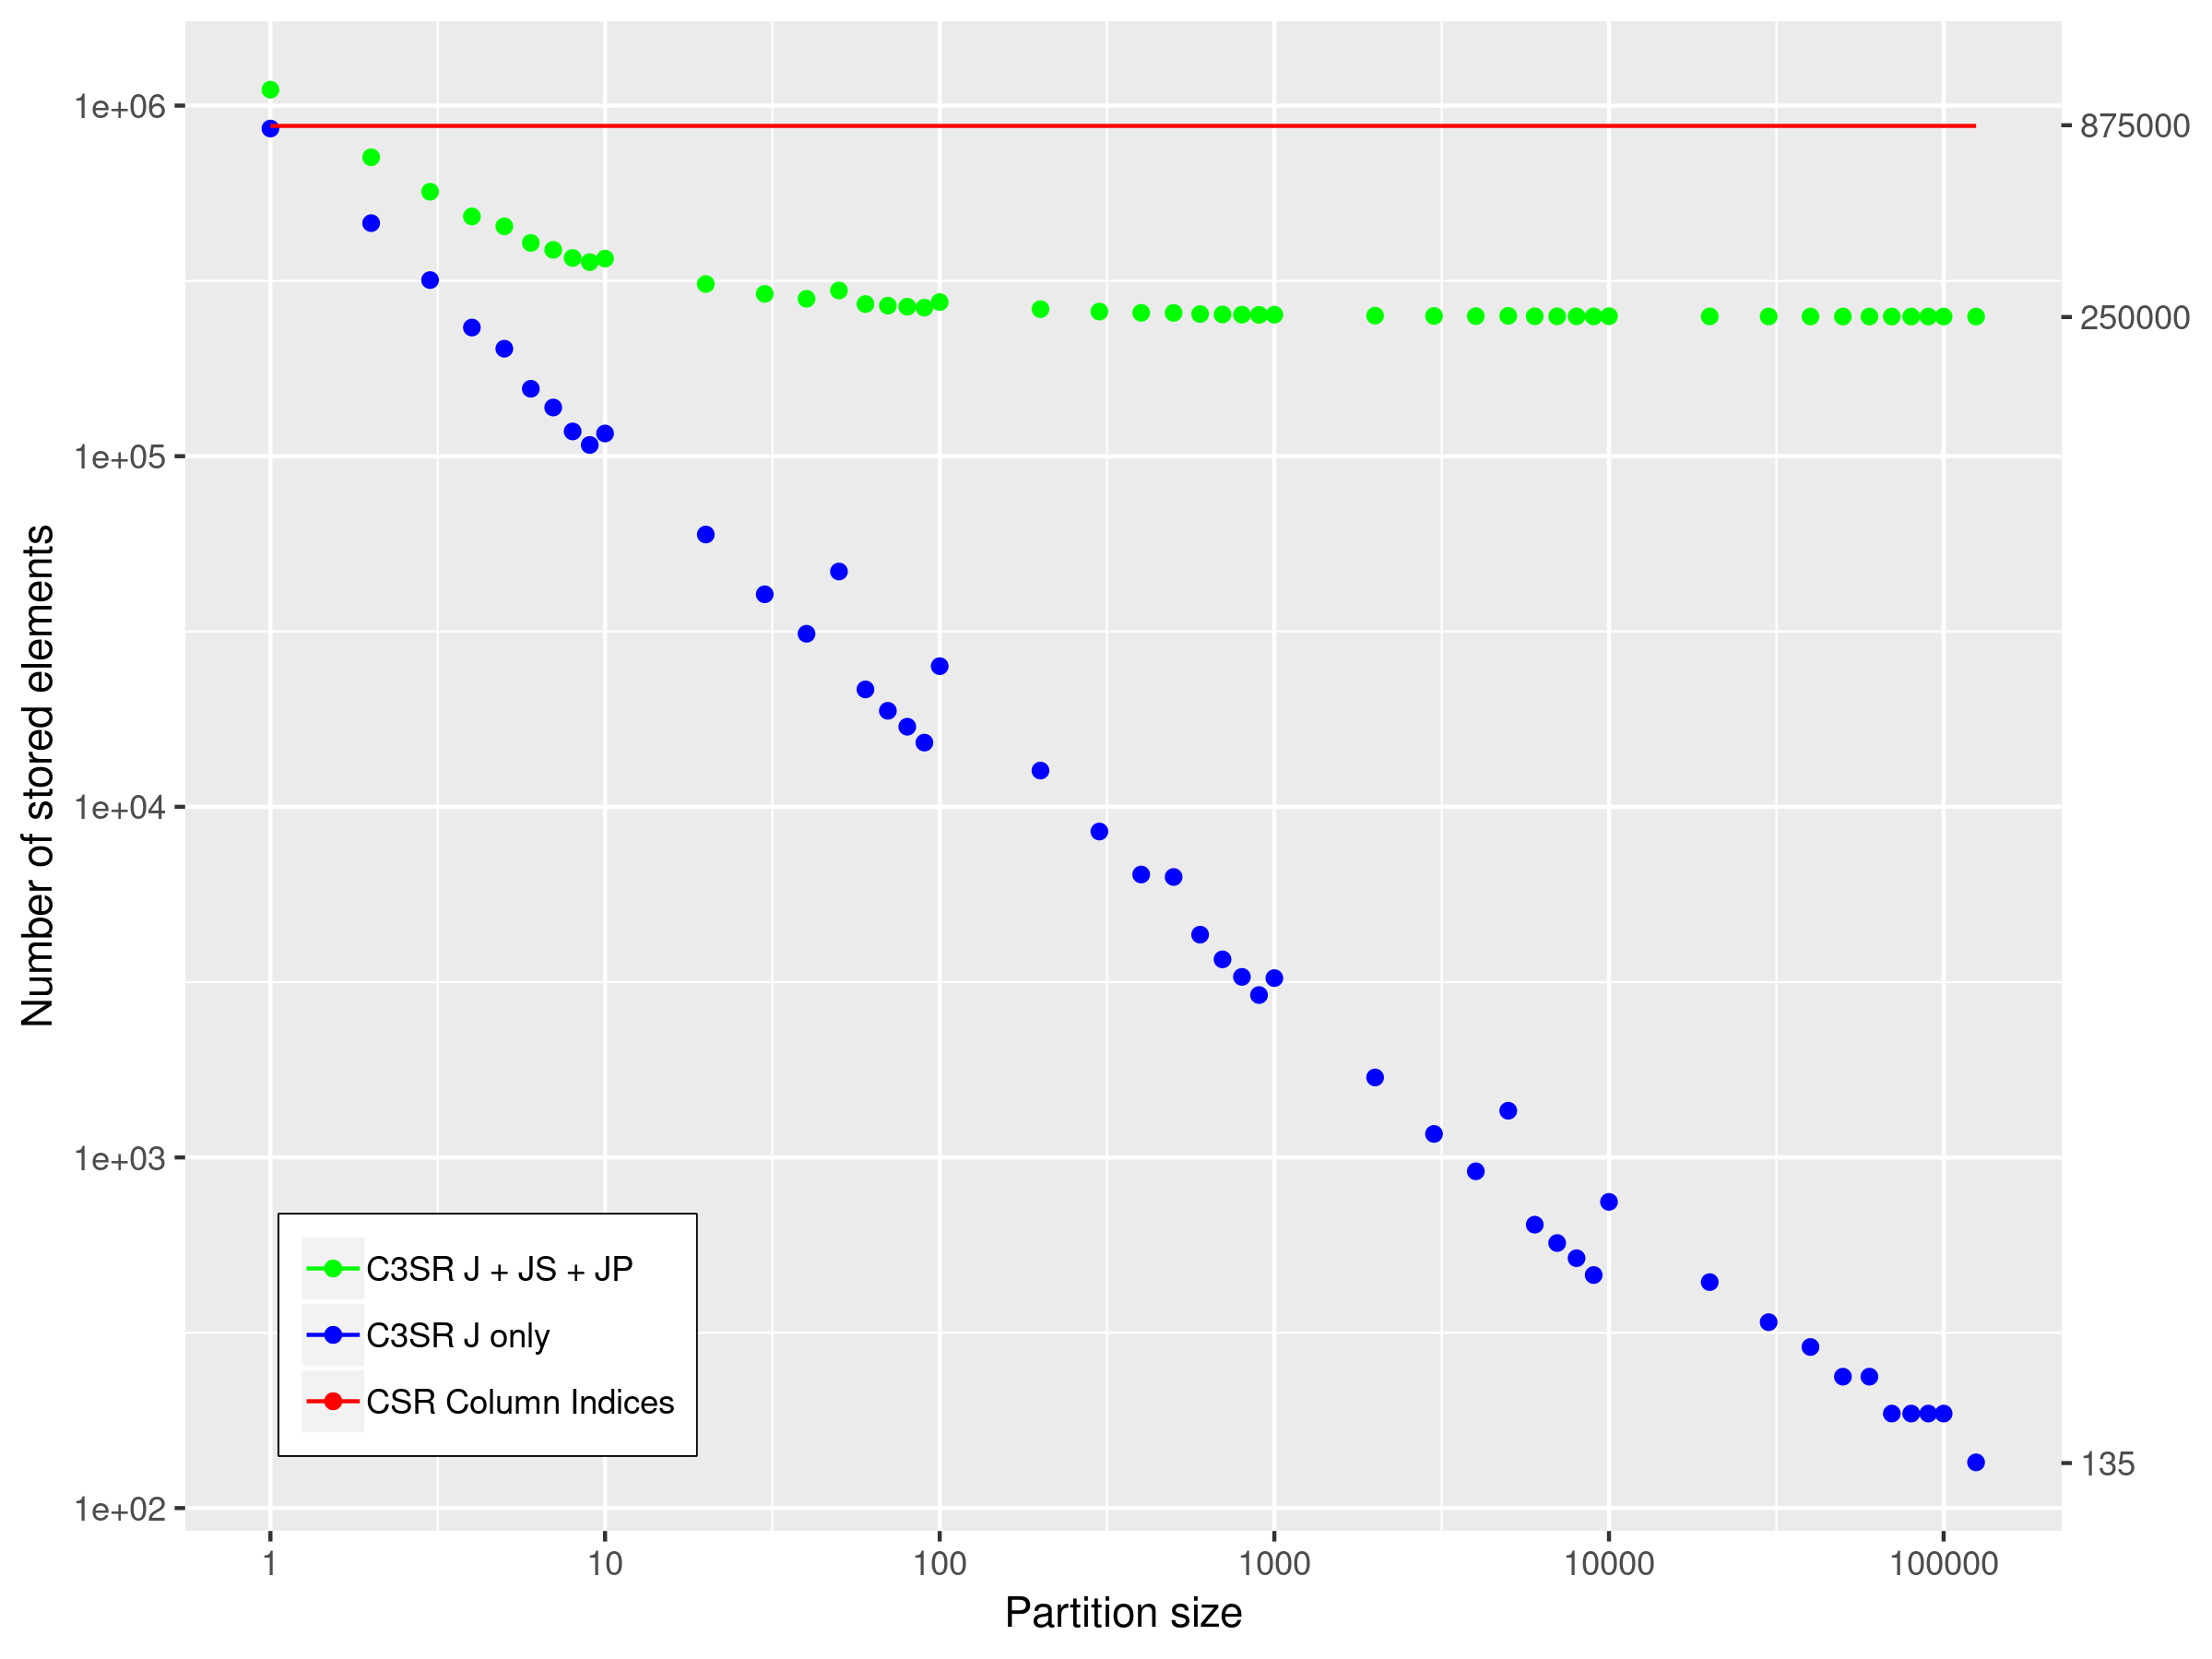
\includegraphics[width=0.8\textwidth]{fig/structural-compression}
      \caption*{TODO}
    \end{figure}

    //TODO: Structural compression mit interleaved matrices
\section{Summary}
  Advantages: General purpose, good performance, parallel scalability
  Disadv: Static structure (cannot add/remove elements)

OVERALLTODO:
  TODO: ... will be referred to as 'structured matrix' ==== adjacency matrix of structured grids assuming xyz-indexing

  "No need to fully compress the matrix" --> Diminishing returns; parallelizability

  TODO:
    - Abschätzung Performance-Gain vs. Speicherzugriffe/Matrixgröße
    - KNL Cores haben simple Hardware --> Effekt von korrektem Code ist größer
    - KNL: Falls Chunks zu groß werden fällt Working Set aus Cache
    - Wozu Partitionierung --> Threads können parallel arbeiten
    - Throughput-Abschätzung (Bewegte Datenmenge aus DRAM / Dauer); A,x,y (jedes Element wird ~1 mal ausgelesen)

\printbibliography
\end{document}
